\documentclass[../main/git_course_main.tex]{subfiles}
\begin{document}
	
	% Figure edits: Update base directory name to "hw_repo"
	
	\setcounter{chapter}{1}
	\chapter{Understanding and using a repository}
	
	\section{Overview}
	
	In this chapter, we will:
	
	\begin{itemize}
		\item Do a quick demonstration of how to set up a repository and add files to it
		\item Introduce important core concepts in Git
		\item Go through the demonstrated commands at a slower pace
	\end{itemize}
	
	\section{Crash and burn}
	
	As a first taste of Git, you will be shown a commonly used sequence of commands that:
	
	\begin{itemize}
		\item \textit{Initializes} a new Git \textit{repository}
		\item Creates some files in the \textit{file tree}
		\item Prepares edited files to be included in the next commit by adding them to the \textit{stage}
		\item Creates a new \textit{commit} based on the staged changes
	\end{itemize}
	
	After running through the commands, we will back up and go through the process step by step, explaining what is going on.
	
	\begin{figure}[h!]
		\begin{redbox}
			It is recommended that you run the commands alongside the material and look for yourself how each command effects your Git repository. \\
			
			You will not always be able trace the state of the repository (and the output) exactly as the text sometimes makes jumps back time to make it possible to illustrate the repository, but you should be able to roughly trace the commands and create your own history.
		\end{redbox}
	\end{figure}
	
	\subsection{Running the commands}
	
	To create a repository within a directory, we use the command \verb$git init$. This initializes a Git repo (repository) within the current working directory.
	
	\begin{codebox}
		\begin{lstlisting}
			$ mkdir MyRepo
			$ cd MyRepo
			$ git init
			Initialized empty Git repository in /home/user/MyRepo/.git/
		\end{lstlisting}
	\end{codebox}
	
	Next, we add two files to the file tree. Let's create a README-file and a "Hello world" script.
	
	\begin{codebox}
		\begin{lstlisting}
			$ echo 'README - Course repository' > README.md
			$ echo '#!/bin/bash' > hello_world.sh
			$ echo 'echo "Hello world"' >> hello_world.sh
		\end{lstlisting}
	\end{codebox}
	
	Next, we decide on which changes to include in the next commit - the next version of the file tree which will be frozen in the history of the repository. In this case, we 
	include both the README and the Hello world-script in the commit.
	
	\begin{codebox}
		\begin{lstlisting}
			$ git add README.md
			$ git add hello_world.sh
		\end{lstlisting}
	\end{codebox}
	
	Finally, we are ready to create a commit including the newly created files.
	
	\begin{codebox}
		\begin{lstlisting}
			$ git commit -m "Creates README and Hello World script"
			[main (root-commit) 086acdf] Creates README and Hello World 
			script
			2 files changed, 3 insertions(+)
			create mode 100644 README.md
			create mode 100644 hello_world.sh
		\end{lstlisting}
	\end{codebox}
	
	Done! Now we have started a repository in our working directory, created a file, and added that file to our repository. The current state of the files is saved in the repository.
	
	The next step here is usually to sync the changes with a remote repository.
	This will be introduced in Chapter 5.
	
	\section{What did just happen? - Terms and concepts}
	
	Now, let's back up a bit. What is actually going on in the repository when running the different commands? Here, we will present some core terms and concepts which makes Git considerably easier to understand. It is worth putting in some extra reading-effort here, as the presented concepts will help you better understanding the different Git commands you will be using.
	
	We will go through:
	
	\begin{itemize}
		\item What a \textit{commit} represents, and which information it contains
		\item How files transition between the \textit{file tree}, the \textit{stage} and the \textit{repository}, and the relationship between them
		\item What \textit{heads} are, and how the \verb$HEAD$ head is special
	\end{itemize}
	
	\subsection{Vocabulary}
	
	To understand a concept you need to know its vocabulary. You will frequently encounter the words presented here in the rest of this material. The concepts are explained in more depth below.
	
	\begin{description}
		\item[file tree] A set of files and directories originating in a particular directory. The subdirectories and files of a directory is its file tree. This is present independently of the version control system.
		\item[commit] A snapshot of a particular state of the \textit{file tree}. A commit contains an ID, the state of the file tree and a reference to its parent commit among with some other information.
		\item[repository] A repository is attached to a \textit{file tree}. Commits representing changes to its \textit{file tree} are saved in the \textit{repository}.
		\item[staging area / index] Location used to choose changes that were made to the \textit{file tree} and that should be included in the next \textit{commit}.
		\item[branch] The \textit{commits} of a \textit{repository} can be branched, with multiple features being developed in parallel. This is called \textit{branching} and is a powerful part of Git which will be revisited in Chapter 4.
		\item[heads] References to particular \textit{commits}. \verb$HEAD$ is a \textit{head} referring to the commit currently represented in the \textit{file tree}. \verb$main$ is a \textit{head} commonly referring to the latest commit on the main development branch.
	\end{description}
	
	\subsection{A commit}
	
	A commit takes a snapshot of a particular state of the file tree (which files are present and what their current content is). The commit is actually storing the changes made compared to its parent commit. This can be used together with all parent commits to retrieve the file structure that is represented in this particular snapshot.
	
	A commit contains the following information (this is visualized in Figure \ref{fig:a_commit}):
	
	\begin{itemize}
		\item A unique ID, which can be used to refer to the commit
		\item Information about the commit, which includes the snapshot of the file tree and the descriptive message provided together with the commit
		\item A reference to the parent commit
	\end{itemize}
	
	The ID is an SHA-1 hash based on the content of the commit. It is represented as a 40 character long string. An example is shown in Figure \ref{fig:SHA}.
	Commits are often referred to using only the first 6-7 letters/digits of their IDs.
	
	\begin{figure}[h!]
		\center\verb$74a3f1511429d8b688aad299485546b4cc86cb75$
		\caption{An SHA-1 hash commit ID}
		\label{fig:SHA}
	\end{figure}
	
	The parent commit represents the state of the repository before making the changes in the current commit.
	
	\begin{figure}[h!]
		\centering
		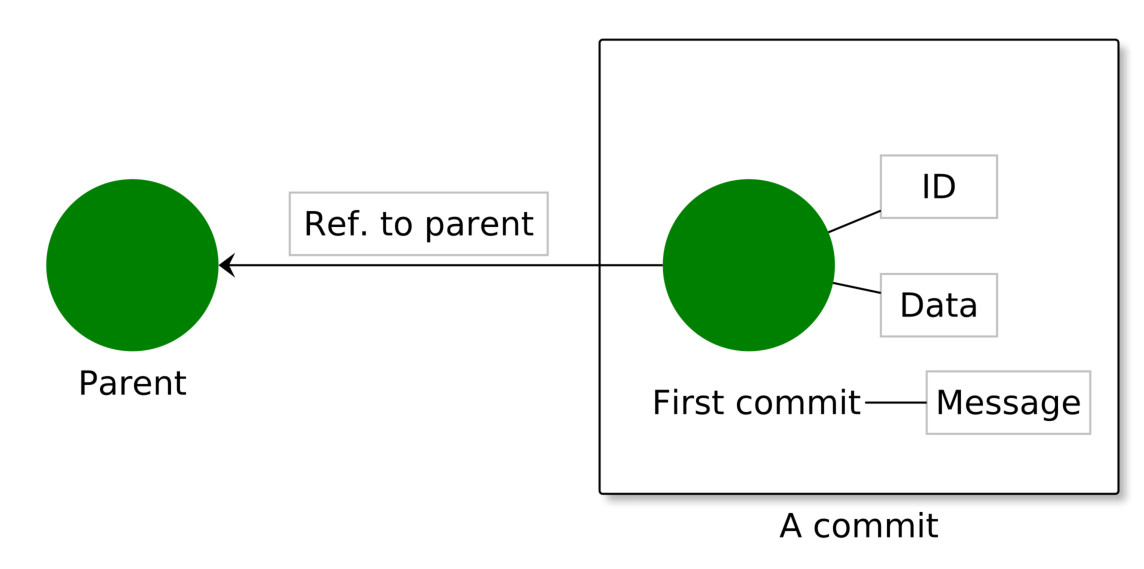
\includegraphics[width=0.8\textwidth]{../visualizations/chapter2/21_the_commit.pdf}
		\caption{A commit consists of three parts. Its ID, a reference to its parent, and its data.}
		\label{fig:a_commit}
	\end{figure}
	
	\subsection{The repository, the file tree and the stage / index}
	
	% More thorougly introduce both heads, HEAD, HEAD^, main, index/stage, repository, file tree
	
	\begin{figure}[h!]
		\centering
		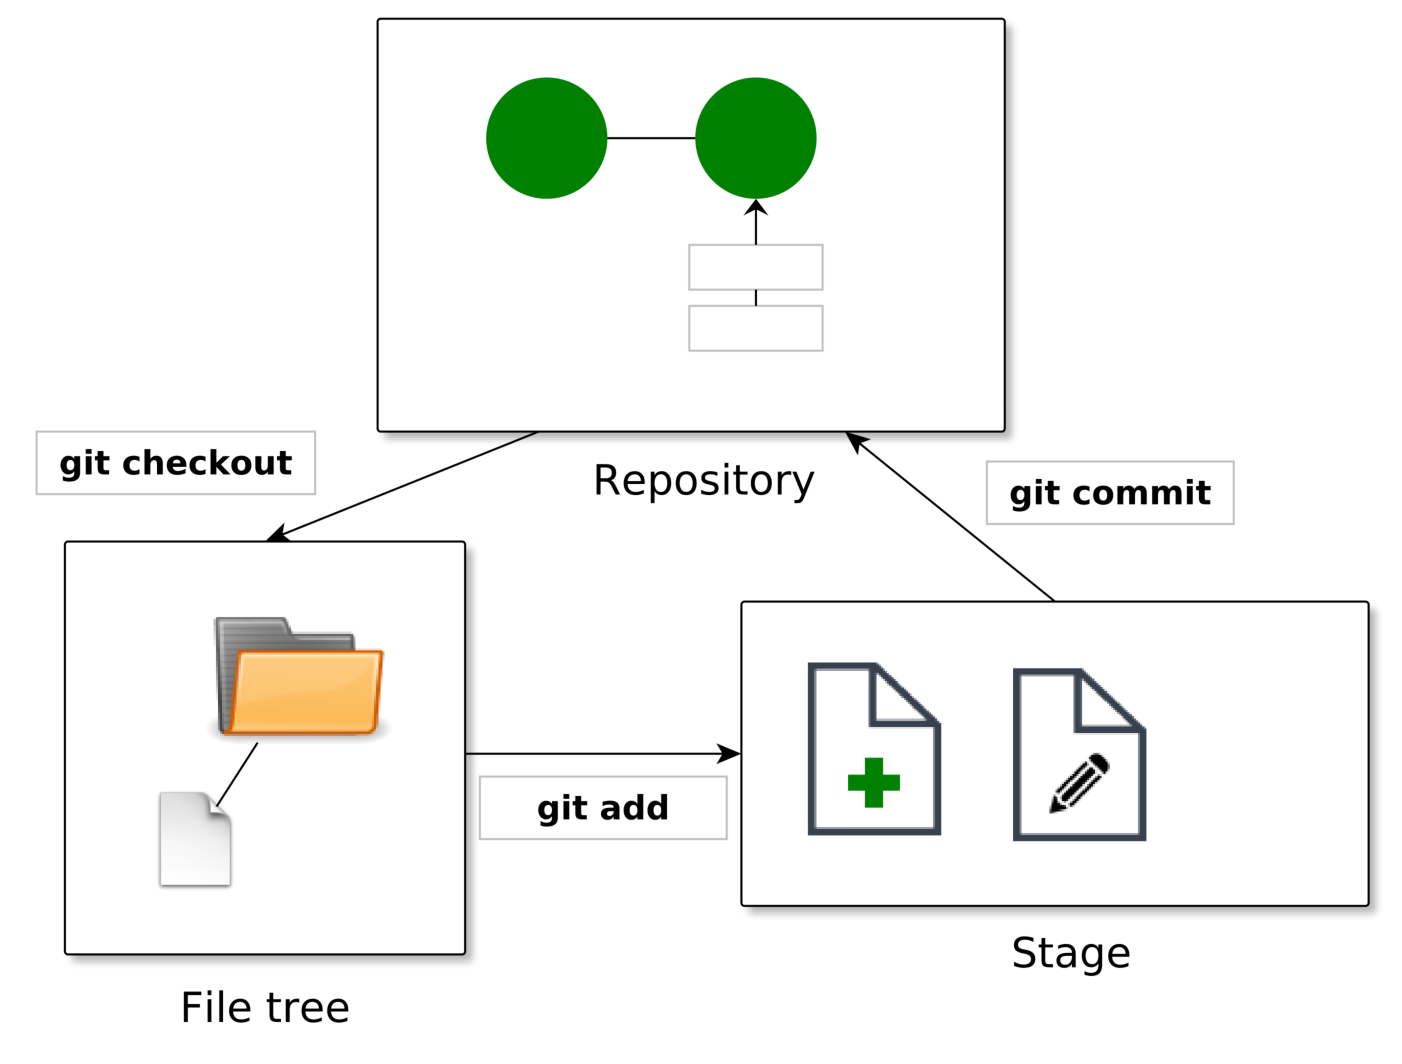
\includegraphics[width=0.8\textwidth]{../visualizations/chapter2/22_visualize_stage_file_system_and_repo.pdf}
		\caption{The three major entities in the Git system}
		\label{fig:repo_filetree_stage}
	\end{figure}
	
	When working with Git, you constantly interact with the file tree, the stage and the repository.
	
	You are used to the \textit{file tree}. It is simply the structure of files and directories which you use everyday when not using Git.
	
	The \textit{stage} is a place to which you add the changes you want to include in your next commit. You don't need to include all the changes made to the
	file tree in a particular commit. The history is easier to read if you include changes related to a particular feature in one commit.
	
	The repository is the system keeping track of all the commits. Every time you make a new commit (based on the staged file-changes), it is added to the repository.
	
	\subsection{The concept of \textit{heads}}
	
	\begin{figure}[h!]
		\centering
		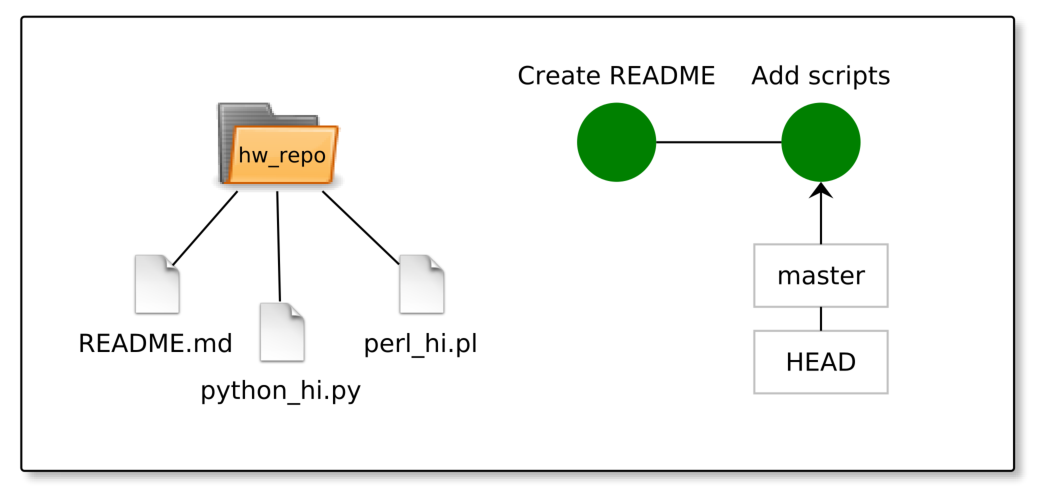
\includegraphics[width=0.8\textwidth]{../visualizations/chapter2/c25_repo_second_commit.pdf}
		\caption{A file tree and repository with the heads "HEAD" and "main"}
		\label{fig:head_illustration}
	\end{figure}
	
	Heads are used in Git to refer to particular commits. They are used to keep track of the leading commits of branches, and for keeping track of which commit that is currently represented in the file tree (the \verb$HEAD$). In Figure \ref{fig:head_illustration} the heads \verb$HEAD$ and \verb$main$ are both pointing to the second commit.
	
	When creating an empty repository, you always get two heads: \verb$main$ and \verb$HEAD$. When we later on make branches for our repository, we will create one new head per branch.
	
	\begin{enumerate}
		\item[main] Generally the central development branch, where we insert changes that we want to include in the official versions of the code / text. In older versions also called "master".
		\item[HEAD] Special head pointing to the currently active commit. We can investigate the file tree of different commits by moving the \verb$HEAD$ to the corresponding commit. This is further investigated in Chapter 3.
	\end{enumerate}
	
	We will later on move \verb$HEAD$ to different commits, which changes the file tree to the one represented by that commit.
	
	\subsection{Concept-recap}
	
	Before leaving this section, make sure that you have an idea of the following concepts:
	
	\begin{itemize}
		\item What a commit represents, and which information it contains.
		\item The file tree, the stage and the repository, and how they are related.
		\item What heads are, and how the \verb$HEAD$ head is special.
	\end{itemize}
	
	\section{Creating a new repository, slowly...}
	
	% Some theoretical discussion
	% Visualize as both files and some commits?
	% Terms: head, HEAD, main
	% Commands: git init/status/add/commit
	
	%The example-repository used throughout this material is found on GitHub (the setup of the hosting is shown in chapter 4). Here, you can browse the files
	%and all the commits. \\
	%
	%\url{https://github.com/Jakob37/GitCourse-HelloWorlds} \\
	
	\subsection{Creating the repository - First steps}
	
	As a first step, let's create a directory called \verb$hw_repo$ (for "Hello World repository") which we will use for our project, and change our working directory to that directory (use a more descriptive name when not constrained by the page width of your teaching material). 
	At this point, our folder contains an empty file tree, and no repository or stage.
	
	\begin{figure}[h!]
		\begin{redbox}
			It might be a good idea to follow along and start a new repository here.
			Practice makes perfect...
		\end{redbox}
	\end{figure}
	
	\begin{codebox}
		\begin{lstlisting}
			$ mkdir hw_repo
			$ cd hw_repo
		\end{lstlisting}
	\end{codebox}
	
	Next, we initialize the repository within the folder. This will create a (hidden) folder named \verb$.git$ containing the repository.
	
	\begin{codebox}
		\begin{lstlisting}
			$ git init
			Initialized empty Git repository in /home/user/hw_repo/.git/
		\end{lstlisting}
	\end{codebox}
	
	\begin{figure}[h!]
		\begin{bluebox}
			Command: \verb$git init$ \\
			
			Initializes a new repository within the current file tree. The repository is related to the current working directory and its subdirectories.
		\end{bluebox}
		\label{command:init}
		\caption{git init - Initialize a new repository}
	\end{figure}
	
	At this point the directory only contains the hidden \verb$.git$-folder containing the repository files. This is shown in Figure \ref{fig:dot_git}.
	
	\begin{figure}[h]
		\centering
		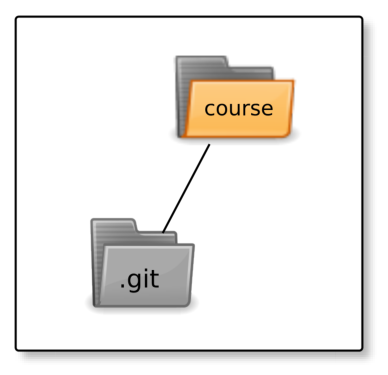
\includegraphics[width=0.4\textwidth]{../visualizations/chapter2/c23_hidden_folder_in_git.pdf}
		\caption{The file system of a newly initialized repository. The gray folder is hidden, and will not be shown in the rest of the figures.}
		\label{fig:dot_git}
	\end{figure}
	
	\section{Saving changes in a commit}
	
	Now, let's create a README file, add it to the stage and commit it to the repository. To do this we'll need to introduce two new commands:
	\verb$git add$ and \verb$git commit$.
	
	First, we create a new file within the file tree. We use the \verb$echo$ command to create the readme \verb$README.md$ containing the line \verb$'A Hello World collection'$. The \verb$README.md$ file is used on services like GitHub to display a README for the repository on the site.
	
	\begin{codebox}
		\begin{lstlisting}
			$ echo 'A Hello World collection' > README.md
		\end{lstlisting}
	\end{codebox}
	
	We can at any time see the status of the repository using the command \verb$git status$.
	This gives us (among other things) information about changes made to the file tree and which files that are staged and ready to be committed.
	
	\begin{codebox}
		\begin{lstlisting}
			$ git status
			On branch main
			
			Initial commit
			
			Untracked files:
			(use "git add <file>..." to include in what will 
			be committed)
			README.md
			nothing added to commit but untracked files present 
			(use "git add" to track)
		\end{lstlisting}
	\end{codebox}
	
	This tells us that:
	
	\begin{enumerate}
		\item The current branch is \verb$main$
		\item It is the first commit of the repository ("Initial commit")
		\item We have one new file in the file tree which isn't tracked by the repository - \verb$README.md$
		\item There are currently no staged files
	\end{enumerate}
	
	Let's add \verb$README.md$ to the stage using \verb$git add$, and check the status again.
	
	\begin{codebox}
		\begin{lstlisting}
			$ git add README.md
			$ git status
			On branch main
			
			Initial commit
			
			Changes to be committed:
			(use "git rm --cached <file>..." to unstage)
			
			new file:   README.md
		\end{lstlisting}
	\end{codebox}
	
	Now, the status looks slightly different. We don't have any untracked files in the file tree. We have one file (\verb$README.md$) ready to be committed. The staged changes ready to be committed are visualized in Figure \ref{fig:first_stage}.
	
	\begin{figure}[h!]
		\centering
		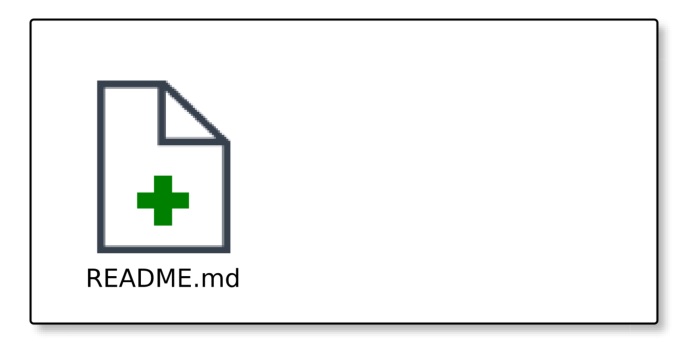
\includegraphics[width=0.6\textwidth
		]{../visualizations/chapter2/241_stage_created_readme.pdf}
		\caption{Stage after adding the newly created README.md}
		\label{fig:first_stage}
	\end{figure}
	
	When doing a commit, we must always supply a commit message describing what the purpose of the changes made in the
	commit is. We can supply the commit description using the \verb$-m$ flag. 
	When running \verb$git commit$ without the \verb$-m$ flag, a default text editor will automatically be opened.
	
	\begin{codebox}
		\begin{lstlisting}
			$ git commit -m "Create README"
			[main (root-commit) b58c6c3] Create README
			1 file changed, 1 insertion(+)
			create mode 100644 README.md
			$ git status
			On branch main
			nothing to commit, working directory clean
		\end{lstlisting}
	\end{codebox}
	
	We have our first commit! Also, there are no untracked changes in the file system and no staged changes.
	The current state of this file tree / repository is visualized in Figure \ref{fig:first_commit}. At this point, we have initialized two heads: \verb$main$ and \verb$HEAD$. They both point to our latest and only commit.
	
	\begin{figure}[h]
		\centering
		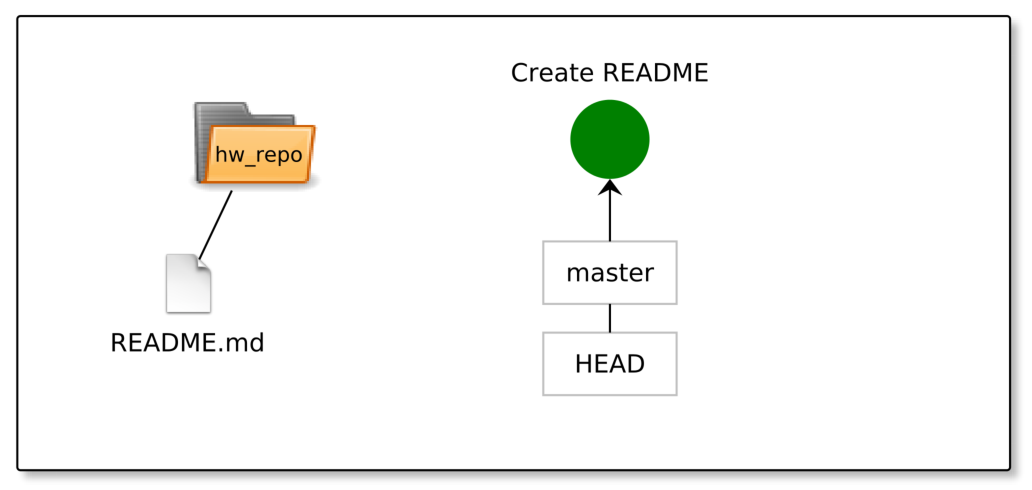
\includegraphics[width=0.8\textwidth]{../visualizations/chapter2/c24_repo_first_commit.pdf}
		\caption{The state of the file system (left) and the repository (right) after the first commit}
		\label{fig:first_commit}
	\end{figure}
	
	\begin{figure}[h!]
		\begin{redbox}
			It is considered good practice to write commit messages in \textit{present tense},
			"Create README" rather than "Created README" or "Creates README".
			
			Although, the most important practice when it comes to commit messages is to write
			clear and descriptive messages. The commit messages used in this material are in
			many cases \textit{not} good examples of descriptive messages - They are kept shorter than usual to fit into text boxes and figures.
		\end{redbox}
	\end{figure}
	
	%%%% GIT ADD %%%%%
	\begin{figure}[h!]
		\begin{bluebox}
			Command: \verb$git add [-A] <path>$ \\
			
			Stages changes made to the file tree. The \verb$-A$ flag can be used to stage files removed from the repository.
			If used \textit{with} the \verb$-A$, moved files and removed files can also be staged.
			It can be used to stage specific files, or directories. When staging directories, all sub-files are
			included.
		\end{bluebox}
		\label{command:add}
		\caption{git add - Stage changes made to the file tree}
	\end{figure}
	%%%%%%%%%%%%%%%%%%%
	
	%%%% GIT COMMIT %%%%%
	\begin{figure}[h!]
		\begin{bluebox}
			Command: \verb$git commit [-m <message>]$ \\
			
			Commits a set of changes to the history, taking a snapshot of the current state of the repository.
			It is required to supply a commit message together with the commit. This commit message should describe the meaning of the commit. It can either be supplied using the \verb$-m$ flag or in the text editor which automatically opens when the command is run without the flag. 
		\end{bluebox}
		\label{command:commit}
		\caption{git commit - Create a snapshot implementing changes added to the stage}
	\end{figure}
	%%%%%%%%%%%%%%%%%%%%%%
	
	%%%% GIT STATUS %%%%%
	\begin{figure}[h!]
		\begin{bluebox}
			Command: \verb$git status$ \\
			
			Prints the current status of the repository. Gives information about changed files
			and which files that are staged and ready to be committed. When working with remotes,
			also provides information about if the local repository is synced with the remote.
		\end{bluebox}
		\label{command:commit}
		\caption{git commit - Create a snapshot implementing changes added to the stage}
	\end{figure}
	%%%%%%%%%%%%%%%%%%%%%%
	
	\newpage
	\section{Committing changes and checking status}
	
	Up until now we have only added files to our file-tree. We can also include file edits in commits. This section will demonstrate how the stage can be useful to pick a set of changes to include into a particular commit.
	
	We make three edits to the file tree:
	
	\begin{itemize}
		\item We add another line to the README
		\item We create a Python Hello world script
		\item We create a Perl Hello world script
	\end{itemize}
	
	\begin{codebox}
		\begin{lstlisting}
			$ echo 'Hello World in different languages' >> README.md
			
			# Let's create hello world in Python
			$ echo '#!/usr/bin/python3' > python_hi.py
			$ echo 'print("Hello world")' >> python_hi.py
			
			# Let's create hello world in Perl
			$ echo '#!/usr/bin/perl' > perl_hi.pl
			$ echo 'print("Hello world");' >> perl_hi.pl
		\end{lstlisting}
	\end{codebox}
	
	Next, we check the status for the repository.
	
	\begin{codebox}
		\begin{lstlisting}
			$ git status
			On branch main
			Changes not staged for commit:
			(use "git add <file>..." to update what will be committed)
			(use "git checkout -- <file>..." to discard changes in 
			working directory)
			
			modified:   README.md
			
			Untracked files:
			(use "git add <file>..." to include in what will be 
			committed)
			
			perl_hi.pl
			python_hi.py
			
			no changes added to commit (use "git add" and/or "git commit 
			-a")
		\end{lstlisting}
	\end{codebox}
	
	At this point we have a number of unstaged changes. The repository sees that \verb$README.md$
	has been modified. It also recognizes \verb$perl_hi.pl$ and \verb$python_hi.py$ as two new untracked files.
	
	To keep the history of the commits nice and tidy, let's commit the 'Hello world' scripts separately from the edit made to \verb$README.md$. Then, we can decide on what to do with the changes made to \verb$README.md$. To do this, we stage only the Hello World-scripts.
	
	\begin{codebox}
		\begin{lstlisting}
			$ git add perl_hi.pl
			$ git add python_hi.py
			$ git status
			On branch main
			Changes to be committed:
			(use "git reset HEAD <file>..." to unstage)
			
			new file:   perl_hi.pl
			new file:   python_hi.py
			
			Changes not staged for commit:
			(use "git add <file>..." to update what will be committed)
			(use "git checkout -- <file>..." to discard changes in 
			working directory)
			
			modified:   README.md
		\end{lstlisting}
	\end{codebox}
	
	Git tells us that the two Hello world scripts are ready to be committed. The staged changes are visualized in Figure \ref{fig:second_stage}. We are now ready to commit
	the addition of the two "Hello world"-scripts. The edit of the \verb$README.md$
	files is not staged, and will not be included in this commit.
	
	\begin{figure}[h!]
		\centering
		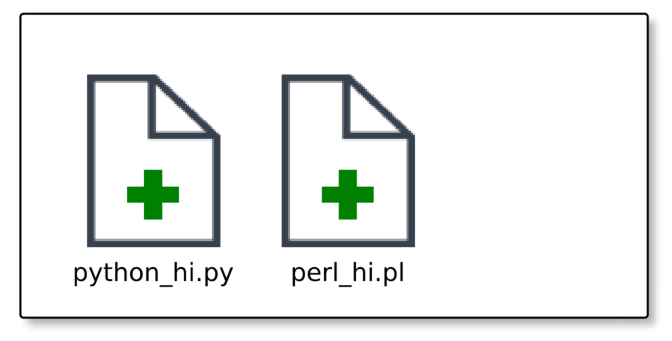
\includegraphics[width=0.6\textwidth
		]{../visualizations/chapter2/251_stage_created_scripts.pdf}
		\caption{Stage after adding two newly created hello-world scripts}
		\label{fig:second_stage}
	\end{figure}
	
	\begin{codebox}
		\begin{lstlisting}
			$ git commit -m "Add scripts"
			[main 7100d36] Add scripts
			2 files changed, 4 insertions(+)
			create mode 100644 perl_hi.pl
			create mode 100644 python_hi.py
			$ git status
			On branch main
			Changes not staged for commit:
			(use "git add <file>..." to update what will be committed)
			(use "git checkout -- <file>..." to discard changes in 
			working directory)
			
			modified:   README.md
			
			no changes added to commit (use "git add" and/or "git commit 
			-a")
		\end{lstlisting}
	\end{codebox}
	
	The file tree and repository after doing this second commit is shown in Figure \ref{fig:second_commit}. We are committing the the \verb$main$ head, which now points to our latest commit. The \verb$HEAD$ head has also switched to the latest commit.
	
	\begin{figure}[h!]
		\centering
		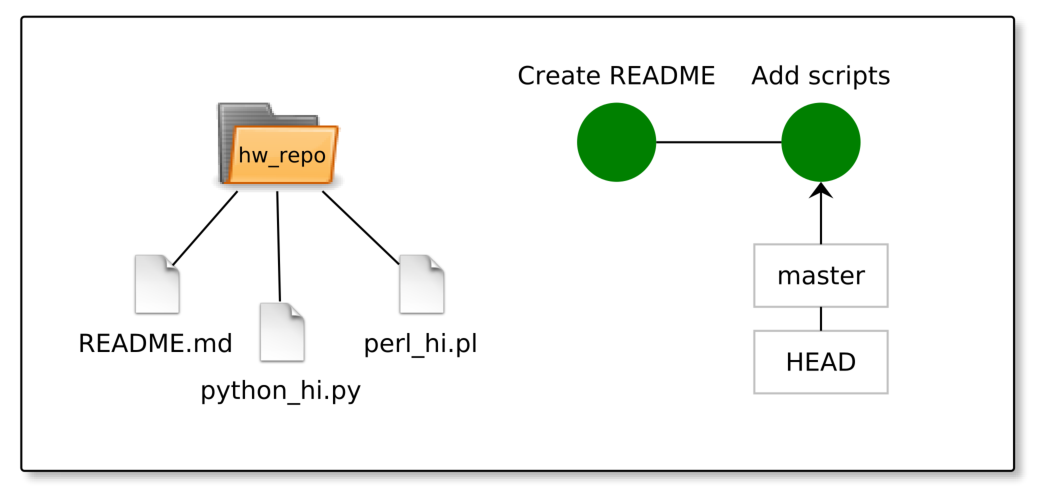
\includegraphics[width=0.8\textwidth]{../visualizations/chapter2/c25_repo_second_commit.pdf}
		\caption{The state of the file system and repository after the second commit}
		\label{fig:second_commit}
	\end{figure}
	
	What do we want to do with the edits to \verb$README.md$? We get some hints by the \verb$git status$ output. If we want to reset it to the state of the last commit, we can run \verb$git checkout$ for that particular file (we will come back to \verb$git checkout$). In this case, we want to keep the changes. So, we stage them and commit them.
	
	\begin{codebox}
		\begin{lstlisting}
			$ git add README.md
		\end{lstlisting}
	\end{codebox}
	
	At this point the changes previously made to \verb$README.md$ are staged, shown in Figure \ref{fig:third_stage}.
	
	\begin{figure}[h!]
		\centering
		
\includegraphics[width=0.6\textwidth]{../visualizations/chapter2/261_stage_modified_readme.pdf}
		\caption{Staged modifications to README.md}
		\label{fig:third_stage}
	\end{figure}
	
	\begin{codebox}
		\begin{lstlisting}
			$ git commit -m "Update README"
			[main 6ab7792] Update README
			1 file changed, 1 insertion(+)
		\end{lstlisting}
	\end{codebox}
	
	Figure \ref{fig:third_commit} shows the state after staging and committing the changes made to \verb$README.md$.
	
	\begin{figure}[h!]
		\centering
		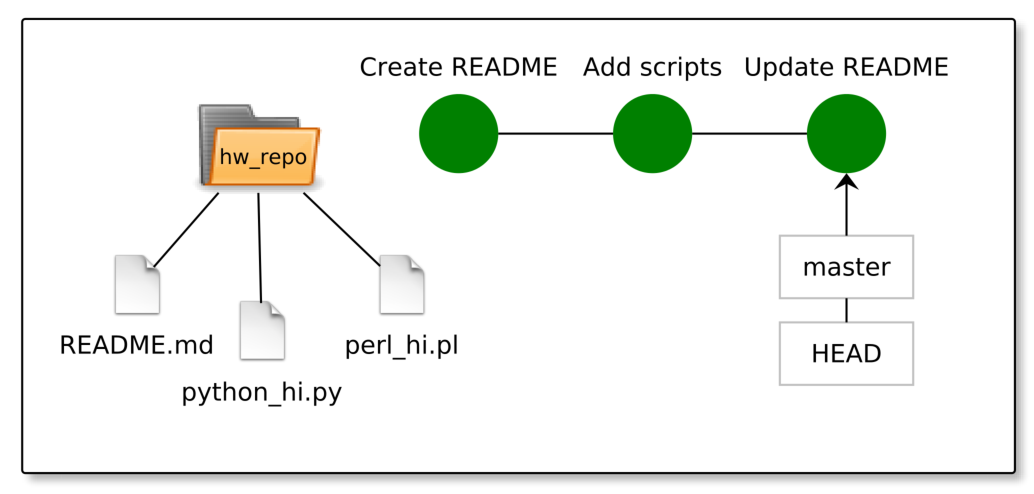
\includegraphics[width=0.8\textwidth]{../visualizations/chapter2/c26_repo_third_commit.pdf}
		\caption{The state of the file system and repository after the third commit}
		\label{fig:third_commit}
	\end{figure}
	
	\section{Staging all the changes}
	
	Changes can always be staged one at a time. Often, it can be useful to stage many files at once. This can be done by supplying a directory to the \verb$git add$ command rather than a specific file. Then all the files contained in that directory are staged.
	
	To stage files starting in your current directory, use the \verb$.$ as argument. (The dot refers to the present working directory in UNIX).
	If you want to stage all files in a Git repository, you can use the \verb$:/$ as argument. This is the "Git-root" - starting from the top directory
	in your Git repository.
	
	\newpage
	\section{Exercises}
	
	Note: You can unstage staged files using the \verb$git reset$ command.
	
	Now, you will independently create a new repository. All the commands needed have been presented in this chapter. If you get stuck, you can take a look at the previous pages.
	
	\subsection{Getting to know the commands}
	
	While running the commands below, trace the current state of the repository using the command \verb$git status$.
	
	\begin{enumerate}
		\item Create an empty directory and initialize a new repository within it.
		\item Create a new file within the directory (\verb$git init$).
		\item Prepare the file for being committing by adding it to the stage (\verb$git add$).
		\item Create your first commit, storing the changes you have made in the repository (\verb$git commit$).
		\item Add multiple files, and try including only some of them in a commit.
		\item Remove one of your files, and include the removal in a commit.
		\item Continue making changes (adding, editing and removing files) to your file tree and commit them to the repository until you feel comfortable using those commands.
	\end{enumerate}
	
	\subsection{Understanding the system}
	
	\begin{enumerate}
		\item Visualize the file tree, the repository, the stage and the heads in the steps done in the previous exercise. Either do this on paper, or simply by thinking in through. How does each of the commands effect the file tree, stage and repository?
	\end{enumerate}
	
	You now know enough to run a fully functioning local Git repository!
	
	\newpage
	\section{Recap}
	
	\subsection{Concepts}
	
	\begin{itemize}
		\item What does a commit represent, and what information does it contain?
		\item What roles do the file tree, the repository and the stage/index have?
		\item What are \textit{heads}, and what are their purpose?
		\item How is the \verb$HEAD$ head special?
	\end{itemize}
	
	\subsection{Commands}
	
	Make sure that you are comfortable with the following commands.
	
	\begin{description}
		\item \verb$git init$
		\item \verb$git add [-A] <path>$
		\item \verb$git commit [-m <message>]$
		\item \verb$git status$
	\end{description}
	
\end{document}
